% Chapter 3

\chapter{Cut-minimal graphs and Cheeger graphs}

\label{Chapter3}

In this chapter we start from the work of Kozlov (see \cite{1}) in which a graph theoretical approach to the first Cheeger constant of a simplex was developed. In the course of this approach the so called cut-minimal graphs appeared, which exactly describe first dimensional cosystoles in a very intuitive way. Beside the benefit for the research on Cheeger constants, we think that exploring cut-minimal graphs could provide interesting structures which might be enlightening and helpful in other braches of combinatorics and topology as well. As a consequence of the first main result of this chapter (Theorem \ref{theorem1}) we will determinine the dimension and partly the homology of a simplicial complex, which contains all information about the cut-minimal graphs on a certain number of vertices. In the second part of this chapter, we face the research on the first Cheeger constant of a simplex by investigating combinatorial properties of the Cheeger graphs which are exactly those cut-minimal graphs that determine this constant.

\section{Cut-minimal graphs}


\subsection{Basic definitions and properties}
The following definition and some words about motivation and intuition for it can be found in \cite{1}.

\begin{defi}
Consider a graph \(G=([n],E)\). For any subsets \(A,B\subset [n]\), define:
\[
E_G(A,B):=\{(v,w)\in E\: :\: v\in A\text{, }w\in B\}
\]
and
\[
NE_G(A,B):=\{(v,w)\notin E\: :\: v\in A\text{, }w\in B\}
\]
A graph \(G=([n],E)\) is called \textbf{cut-minimal}, if for every \(S\subset[n]\) we have
\[
|E_G(S,[n]\setminus S)|\leq |NE_G(S,[n]\setminus S)|,
\]
which is equivalent to
\[
|E_G(S,[n]\setminus S)|\leq\frac{|S|(n-|S|)}{2}.
\]
\end{defi}

Note, that there is a one-to-one correspondence between the graphs on \(n\) vertices and the \(1\)-chains (more precisely the elements of \(C_1(\Delta^{[n]})\)) as follows:\\
For a graph \(G=([n],E)\) set \(c_G:=\sum\limits_{e\in E}e\in C_1(\Delta^{[n]})\) and for a chain \(c\in C_1(\Delta^{[n]})\) set \(G_c:=([n],E)\), with \(E:=supp(c)\). Considering characteristic cochains we also get a one-to-one corresponsing between graphs on \(n\) vertices and \(1\)-cochains and we observe the following relation:

\begin{lem}\label{lemma16}
A graph \(G=([n],E)\) is cut-minimal if and only if the corresponding cochain \(c_G^*\) is a cosystole.
\begin{proof}
%FILL IN PROOF
\end{proof}
\end{lem}

\begin{rem}\label{remark1}
In fact for a graph \(G\) to be cut-minimal we only need to require the preceding condition holding for all \(S\subset [n]\), such that \(1\leq|S|\leq\frac{n}{2}\), since for all \(S\subset [n]\) we have \(E_G(S,[n]\setminus S)=E_G([n]\setminus S,S)\) and \(NE_G(S,[n]\setminus S)=NE_G([n]\setminus S,S)\).
\end{rem}

\begin{expl}
A graph \(G=([n],E)\) forming a circle by the edge set\\
\(E:=\{(i,i+1)\: :\: 1\leq i\leq n-1\}\cup\{(n,1)\}\) is cut-minimal for all \(n\geq 7\) as follows. One can easily see that for all \(S\subset [n]\), such that \(|S|\leq\frac{n}{2}\), we have \(|E_G(S,[n]\setminus S)|\leq 2|S|\) and the inequality \(2|S|\leq\frac{|S|(n-|S|)}{2}\) holds for all \(n\geq |S|+4\), so by \(|S|\leq\frac{n}{2}\) the statement is true for all \(n\geq 7\).
\end{expl}

\begin{defi}
For any \(n,k\in\mathbb{N}\) we define the set of all cut-minimal graphs on \(n\) vertices:
\[
CMG(n):=\{G=([n],E)\: :\: G\text{ is cut-minimal}\},
\]
and its subsets of all cut-minimal graphs on \(n\) vertices and \(k\) edges:
\[
CMG_k(n):=\{G=([n],E)\: :\: G\text{ is cut-minimal and }|E|=k\}.
\]
\end{defi}

\subsection{Maximal cut-minimal graphs}
In \cite{1} there was the simplicial complex \(\mathcal{C}^1(n)\) introduced, constructed as follows:

\begin{itemize}
\item The unordered pairs \((i,j)\) (where \(i,j\in [n]\text{, }i\neq j\)) form the vertices of \(\mathcal{C}^1(n)\).
\item A set of vertices forms a simplex of \(\mathcal{C}^1(n)\), if and only if the corresponding graph is cut-minimal.
\end{itemize}

The complex \(\mathcal{C}^1(n)\) contains all relevant information about the cut-minimal graphs on a certain number of vertices so it might be useful to study its topological and simplicial structure.\\
The first thing to note is that the dimension of \(\mathcal{C}^1(n)\) is obviously one more than the maximal number of edges a cut-minimal graphs can have which obviously coincides with the number \(C_{max}(\Delta^{[n]},1)\) by Lemma \ref{lemma16}.
\\
Let us now determine the number \(C_{max}(\Delta^{[n]},1)\) explicitly.
\begin{prop}\label{proposition3}
\(C_{max}(\Delta^{[n]},1)\geq\binom{\left\lceil\frac{n}{2}\right\rceil}{2}+\binom{\left\lfloor\frac{n}{2}\right\rfloor}{2}\)
\begin{proof}
Let us construct a graph \(G\) on \(n\) vertices as follows. Choose a set \(V'\subset [n]\), such that \(|V'|=\left\lceil\frac{n}{2}\right\rceil\) and connect each pair of vertices from \(V'\) by an edge. Then connect each pair of the remaining \(\left\lfloor\frac{n}{2}\right\rfloor\) vertices by an edge. In other words our graph consists of two complete graphs. If \(n\) is even, they are identical, otherwise they differ by one vertex. In total we get \(\binom{\left\lceil\frac{n}{2}\right\rceil}{2}+\binom{\left\lfloor\frac{n}{2}\right\rfloor}{2}\) edges. We will show that this graph is cut-minimal.\\
Let \(S\subset [n]\) and define \(A:=S\cap V'\) and \(B:=S\setminus A\). If \(n\) is even, we have:
\begin{align}
|E_G(S,[n]\setminus S)|&=|A|(\frac{n}{2}-|A|)+|B|(\frac{n}{2}-|B|)\notag\\
&=\frac{n|A|}{2}-|A|^2+\frac{n|B|}{2}-|B|^2\notag\\
&=\frac{n|S|}{2}-(|A|^2+|B|^2)\notag\\
&\leq\frac{n|S|}{2}-\frac{|S|^2}{2}\notag\\
&=\frac{|S|(n-|S|)}{2},\notag
\end{align}
where the inequality comes from:
\begin{align}
&\quad\quad\quad\:\, (|A|-|B|)^2\geq 0\notag\\
&\Longleftrightarrow\quad |A|^2-2|A||B|+|B|^2\geq 0\notag\\
&\Longleftrightarrow\quad \frac{|A|^2}{2}-|A||B|+\frac{|B|^2}{2}\geq 0\notag\\
&\Longleftrightarrow\quad |A|^2+|B|^2\geq\frac{|A|^2}{2}+|A||B|+\frac{|B|^2}{2}\notag\\
&\Longleftrightarrow\quad |A|^2+|B|^2\geq\frac{|S|^2}{2}.\notag
\end{align}
If \(n\) is odd, we have:
\begin{align}
|E_G(S,[n]\setminus S)|&=|A|(\frac{n+1}{2}-|A|)+|B|(\frac{n-1}{2}-|B|)\notag\\
&=\frac{n|A|}{2}+\frac{|A|}{2}-|A|^2+\frac{n|B|}{2}-\frac{|B|}{2}-|B|^2\notag\\
&=\frac{n|S|}{2}-(|A|^2+|B|^2-\frac{|A|-|B|}{2})\notag\\
&\leq\frac{n|S|}{2}-\frac{|S|^2}{2}\notag\\
&=\frac{|S|(n-|S|)}{2},\notag
\end{align}
where the inequality comes from:
\begin{align}
&\quad\quad\quad\:\, (|A|-|B|)^2-(|A|-|B|)\geq 0\notag\\
&\Longleftrightarrow\quad (|A|-|B|)^2-|A|+|B|\geq 0\notag\\
&\Longleftrightarrow\quad |A|^2+|B|^2-|A|+|B|\geq 2|A||B|\notag\\
&\Longleftrightarrow\quad \frac{|A|^2}{2}+\frac{|B|^2}{2}-\frac{|A|}{2}+\frac{|B|}{2}\geq |A||B|\notag\\
&\Longleftrightarrow\quad |A|^2+|B|^2-\frac{|A|}{2}+\frac{|B|}{2}\geq \frac{|A|^2}{2}+\frac{2|A||B|}{2}+\frac{|B|^2}{2}\notag\\
&\Longleftrightarrow\quad |A|^2+|B|^2-\frac{|A|-|B|}{2}\geq\frac{(|A|+|B|)^2}{2}\notag\\
&\Longleftrightarrow\quad |A|^2+|B|^2-\frac{|A|-|B|}{2}\geq\frac{|S|^2}{2}.\notag
\end{align}
Hence, the constructed graph is cut-minimal.
\end{proof}
\end{prop}
\begin{rem}
For further proofs and calculations it might be helpful to keep mind that we have:
\begin{align}
&\binom{\left\lceil\frac{n}{2}\right\rceil}{2}+\binom{\left\lfloor\frac{n}{2}\right\rfloor}{2}=\frac{n^2-2n+1}{4},&\text{ for }n\text{ odd, and}\notag \\
&\binom{\left\lceil\frac{n}{2}\right\rceil}{2}+\binom{\left\lfloor\frac{n}{2}\right\rfloor}{2}=\frac{n^2-2n}{4},&\text{ for }n\text{ even.}\notag
\end{align}
\end{rem}
\begin{thm}\label{theorem1}
\(C_{max}(\Delta^{[n]},1)=\binom{\left\lceil\frac{n}{2}\right\rceil}{2}+\binom{\left\lfloor\frac{n}{2}\right\rfloor}{2}\)
\begin{proof}
In a cut-minimal graph the maximum degree of each vertex is \(\left\lfloor\frac{n-1}{2}\right\rfloor\), so if \(n\) is even, we have:
\[
C_{max}(\Delta^{[n]},1)\leq\frac{n\left\lfloor\frac{n-1}{2}\right\rfloor}{2}=\frac{n^2-2n}{4}=2\binom{\frac{n}{2}}{2}=\binom{\left\lceil\frac{n}{2}\right\rceil}{2}+\binom{\left\lfloor\frac{n}{2}\right\rfloor}{2}
\]
If \(n\) is odd, the situation becomes more complicated. We only know that
\[
C_{max}(\Delta^{[n]},1)\leq\frac{n\left\lfloor\frac{n-1}{2}\right\rfloor}{2}=\frac{n\frac{n-1}{2}}{2}=\frac{n^2-n}{4},
\]
but in this case unfortunately the right hand side is bigger than \(\binom{\left\lceil\frac{n}{2}\right\rceil}{2}+\binom{\left\lfloor\frac{n}{2}\right\rfloor}{2}\), so we have to find a smaller upper bound for \(C_{max}(\Delta^{[n]},1)\). The following investigation shows, that a graph with \(\frac{n^2-n}{4}\) edges can not be cut-minimal anymore, which will lead to the requested bound.\\
Consider a graph \(G=([n],E)\), and choose a vertex \(v\in [n]\), such that\\
\(\text{deg}_G(v)=\frac{n-1}{2}\). If such a vertex does not exist, we have
\[
|E|\leq\frac{n(\frac{n-1}{2}-1)}{2}=\frac{n^2-3n}{4}<\frac{n^2-2n+1}{4}=\binom{\left\lceil\frac{n}{2}\right\rceil}{2}+\binom{\left\lfloor\frac{n}{2}\right\rfloor}{2}
\]
and we are done. Now there exist exactly \(\frac{n-1}{2}\) vertices \(v_1,\ldots,v_{\frac{n-1}{2}}\in [n]\), such that \((v,v_i)\notin E\), for all \(i=1,\ldots,\frac{n-1}{2}\). If we had \(\text{deg}_G(v_i)=\frac{n-1}{2}\) for one of these vertices, we would get
\[
|E_G(\{v,v_i\},[n]\setminus\{v,v_i\})|=2\frac{n-1}{2}=n-1>n-2=\frac{2(n-2)}{2},
\]
so \(G\) would not be cut-minimal anymore. It follows that the degree of these \(\frac{n-1}{2}\) vertices has to be at least one lower than assumed, so the number of edges has to be at least \(\frac{n-1}{4}\) lower than assumed, which provides the new inequality:
\begin{align}
C_{max}(\Delta^{[n]},1)&\leq\frac{n^2-n}{4}-\frac{n-1}{4}\notag\\
&=\frac{n^2-2n+1}{4}\notag\\
&=\frac{(n-1)^2}{4}\notag\\
&=\binom{\frac{n+1}{2}}{2}+\binom{\frac{n-1}{2}}{2}\notag\\
&=\binom{\left\lceil\frac{n}{2}\right\rceil}{2}+\binom{\left\lfloor\frac{n}{2}\right\rfloor}{2}\notag
\end{align}
Hence, we have \(C_{max}(\Delta^{[n]},1)\leq\binom{\left\lceil\frac{n}{2}\right\rceil}{2}+\binom{\left\lfloor\frac{n}{2}\right\rfloor}{2}\) in general and by Proposition \ref{proposition3} we are done.
\end{proof}
\end{thm}
Note, that the proof of Proposition \ref{proposition3} even contains a description of the shape of a cut-minimal graph with the maximum number of edges, which furthermore provides information about how a top dimensional simplex is embedded in \(\mathcal{C}^1(n)\). Now the following theorem does not only represent a first statement about the homology of \(\mathcal{C}^1(n)\), but even shows that the construction in the proof of Proposition \ref{proposition3} is the only possible shape of such graphs (top dimensional simplices respectively). Let us first define some basic terminology, which we will mainly need in the next section, but it might already be helpful at this point to know exactly what we mean by deleting or adding edges in a graph.
\begin{defi}
For a graph \(G=([n],E)\) and a family of edges \(e_1,\ldots,e_k\in E\) we define the \textbf{deletion} of \(e_1,\ldots,e_k\) in \(G\) as:
\[
G_{e_1,\ldots,e_k}:=([n],E\setminus\{e_1,\ldots,e_k\}).
\]
For a graph \(G=([n],E)\) and a family of edges \(e_1,\ldots,e_k\in NE_G([n],[n])\) we define the \textbf{addition} of \(e_1,\ldots,e_k\) to \(G\) as:
\[
G^{e_1,\ldots,e_k}:=([n],E\cup\{e_1,\ldots,e_k\}),
\]
\end{defi}
\begin{thm}\label{theorem3}
\(H_{C_{max}(\Delta^{[n]},1)-1}(\mathcal{C}^1(n))\cong 0\)
\begin{proof}
We will first show, that a top dimensional simplex in \(\mathcal{C}^1(n)\) can only be represented as a graph of the type we constructed in the proof of Proposition \ref{proposition3}.\\
Let \(n\) be even. If we set \(n=2t+2\), then by the number \(C_{max}(\Delta^{[n]},1)\) and cut-minimality, the graph \(G\) corresponding to a top dimensional simplex in \(\mathcal{C}^1(n)\) must be \(t\)-regular. Furthermore for any three vertices \(v,w,u\in [n]\) by cut-minimality we have:
\[
E_G(\{v,w,u\},[n]\setminus\{v,w,u\})\leq\frac{3(2t-1)}{2}=3t-\frac{3}{2},
\]
so by \(t\)-regularity among any three vertices at least two of them must be adjacent. Now choose a vertex \(v\in [n]\) and set \(A\) to be the set consisting of all vertices, which are not adjacent to \(v\). Then we have \(|A|=t+1\) by \(t\)-regularity and by the preceding result any two vertices in \(A\) have to be adjacent. Thus, \(A\) provides a complete graph on \(t+1\) vertices, so by \(t\)-regularity \([n]\setminus A\) must also provide a complete graph on \(t+1\) vertices. Hence, every top dimensional simplex in \(\mathcal{C}^1(n)\) (for \(n\) even) corresponds to a graph of that shape.\\
Let now \(n\) be odd. If we set \(n=2t+3\), then by the number \(C_{max}(\Delta^{[n]},1)\) and cut-minimality there exist at least \(t+2\) vertices having degree \(t+1\). Let \(A\) denote the set of these vertices. For any \(v,w\in A\) we have:
\[
E_G(\{v,w\},[n]\setminus\{v,w\})\leq\frac{2(2t+3-2)}{2}=2t+1<2t+2=\text{deg}_G(v)+\text{deg}_G(w),
\]
so all vertices from \(A\) are adjacent. By cut-minimality again we have \(|A|=t+2\), so \(A\) provides a complete graph on \(t+2\) vertices. The number of remaining edges \(\binom{t+1}{2}\) shows, that the remaining \(t+1\) vertices must also provide a complete graph, which is disjoint from the first one, because any other constellation would destroy cut-minimality. So, again every top dimensional simplex in \(\mathcal{C}^1(n)\) corresponds to a graph of the requested type.\\
Now we see that deleting an edge from such a graph (which is the same as deleting a vertex from a top dimensional simplex) produces a graph corresponding to a simplex which appears as a face of one top dimensional simplex, but can not be a face of another top dimensional simplex, since we can not construct a graph of the requested type by adding an edge at any other place than the place where we just deleted it. So, all top dimensional simplices are at most connected via simplices of codimension 2, which implies that \(\mathcal{C}^1(n)\) can be continiously retracted to a complex of codimension 1 and so homology in top dimension vanishes.
\end{proof}
\end{thm}
\begin{defi}
A cut-minimal graph \(G=([n],E)\) is called \textbf{maximal}, if for all\\
\(e\in NE_G([n],[n])\) the addition \(G^e\) is not cut-minimal. We denote the set of all maximal cut-minimal graphs on \(n\) vertices by \(MAX(n)\).
\end{defi}
Since a deletion of a cut-minimal graph is cut-minimal itself, it turnes out that we only have to determine all maximal cut-minimal graphs to find all cut-minimal graphs.
\begin{defi}
Two graphs \(G=([n],E)\) and \(G'=([n],E')\) are called \textbf{isomorphic}, if there exists a map \(f:[n]\rightarrow [n]\), such that \((i,j)\in E\) if and only if \((f(i),f(j))\in E'\).
\end{defi}
\begin{rem}
Note, that an isomorphism of graphs preserves all properties, which are studied in this chapter, especially cut-minimality and the constant \(h(G)\), studied in the next section.
\end{rem}
Figure \ref{figure1:Figure 2} illustrates, how the isomorphism classes of cut-minimal graphs on \(6\) vertices are arranged, where the connecting lines represent the relations between the classes refering to the deletion or addition of edges. Note, that the choosen representatives in the figure do not always satisfy the property of being a deletion or an addition of the shown representative of a class below or above, but in this case there is always another representative in the class which does. We see that beside the class of maximal cut-minimal graphs constructed in the proof of Proposition \ref{proposition3}, we have three more classes of maximal cut-minimal graphs here.

\begin{figure}[ht]
\centering
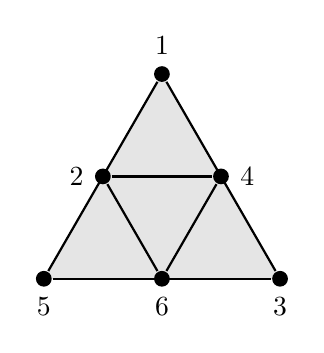
\begin{tikzpicture}[
       thick,
       acteur/.style={
         circle,
         fill=black,
         thick,
         inner sep=2pt,
         minimum size=0.2cm
       }
     ] 

	   \fill[fill=gray!20] (0,0)--(3,0)--(1.5,2.6);

       \node (a1) at (0,0) [acteur,label=below:5]{};
       \node (a2) at (3,0)[acteur,label=below:3]{}; 
       \node (a3) at (1.5,2.6) [acteur,label=above:1]{}; 
       \node (a4) at (0.75,1.3) [acteur,label=left:2]{}; 
       \node (a5) at (2.25,1.3) [acteur,label=right:4]{}; 
       \node (a6) at (1.5,0) [acteur,label=below:6]{};
  
       \draw (a1) -- (a2); 
       \draw (a2) -- (a3); 
       \draw (a1) -- (a3);
       
       \draw (a4) -- (a5);
       \draw (a5) -- (a6);
       \draw (a4) -- (a6);

\end{tikzpicture}
  \caption{The support of a $2$-Cheeger cosystole (The gray triangles represent the four $2$-simplices)}
  \label{figure1:Figure 1}
\end{figure}


Except for the maximal cut-minimal graphs with maximum number of edges we do not know anything about the remaining classes of cut-minimal graphs until now. The following statements now approach this challenge by providing new classes of cut-minimal graphs in general which do not appear as deletions of those largest maximal cut-minimal graphs.

\newpage

\begin{lem}\label{lemma8}
Let \(u_1,\ldots,u_t,s_1,\ldots,s_t\in\mathbb{N}\cup\{0\}\), such that for all \(i=1,\ldots,t\) we have:
\[
u_i+s_i\leq\sum_{\begin{subarray}{l}j=1\\ j\neq i\end{subarray}}^tu_j+s_j,
\]
then we have:
\[
\sum\limits_{i=1}^ts_i(u_i-\sum_{\begin{subarray}{l}j=1\\ j\neq i\end{subarray}}^tu_j)\leq 0
\]
\begin{proof}
If we have
\[
u_i\leq\sum_{\begin{subarray}{l}j=1\\ j\neq i\end{subarray}}^tu_j
\]
for all \(i=1,\ldots,t\), then we are done, since all \(u_i\)'s and \(s_i\)'s are positive. So, let there exist a \(k\in[t]\), such that
\[
u_k>\sum_{\begin{subarray}{l}j=1\\ j\neq k\end{subarray}}^tu_j.
\]
Obviously, there is at most one unique \(u_k\) satisfying this property. Now for all \(i\neq k\) we have:
\[
u_i-\sum_{\begin{subarray}{l}j=1\\ j\neq i\end{subarray}}^tu_j\leq -(u_k-\sum_{\begin{subarray}{l}j=1\\ j\neq k\end{subarray}}^tu_j),
\]
and furthermore we have
\[
s_k<\sum_{\begin{subarray}{l}j=1\\ j\neq k\end{subarray}}^ts_j
\]
by assumption and so we get:
\[
\sum_{\begin{subarray}{l}i=1\\ i\neq k\end{subarray}}^ts_i(u_i-\sum_{\begin{subarray}{l}j=1\\ j\neq i\end{subarray}}^tu_j)\leq-s_k(u_k-\sum_{\begin{subarray}{l}j=1\\ j\neq k\end{subarray}}^tu_j).
\]
Hence, we have:
\[
\sum\limits_{i=1}^ts_i(u_i-\sum_{\begin{subarray}{l}j=1\\ j\neq i\end{subarray}}^tu_j)\leq 0.
\]
\end{proof}
\end{lem}
\begin{prop}
Let \(G=([n],E)\) be a simple graph and let the largest connected component of \(G\) not contain more than \(\frac{n}{2}\) vertices. Then \(G\) is cut-minimal.
\begin{proof}
Let \(C_1,\ldots,C_t\subset [n]\) be the connected components of \(G\) and let \(S\subset [n]\), \(S_i:=S\cap C_i\) and \(U_i:=C_i\setminus S_i\). Then we have:
\[
|E_G(S,[n]\setminus S)|\leq\sum\limits_{i=1}^t|S_i||U_i|
\] 
and
\[
|NE_G(S,[n]\setminus S)|\geq\sum\limits_{i=1}^t(|S_i|\sum_{\begin{subarray}{l}j=1\\ j\neq i\end{subarray}}^t|U_j|).
\]
So, we have to show that
\[
\sum\limits_{i=1}^t|S_i||U_i|\leq\sum\limits_{i=1}^t(|S_i|\sum_{\begin{subarray}{l}j=1\\ j\neq i\end{subarray}}^t|U_j|),
\]
which is equivalent to
\[
\sum\limits_{i=1}^t|S_i|(|U_i|-\sum_{\begin{subarray}{l}j=1\\ j\neq i\end{subarray}}^t|U_j|)\leq 0,
\]
but this follows directly from Lemma \ref{lemma8}, since by the assumption \(|C_i|\leq\frac{n}{2}\) for all \(i\), we have:
\[
|S_i|+|U_i|=|C_i|\leq\sum_{\begin{subarray}{l}j=1\\ j\neq i\end{subarray}}^t|C_j|=\sum_{\begin{subarray}{l}j=1\\ j\neq i\end{subarray}}^t|S_j|+|U_j|.
\]
\end{proof}
\end{prop}

Let us now define and determine the counterpart of the number \(C_{max}(\Delta^{[n]},1)\), namely the minimal number of  edges, a non-cut-minimal graph can have.
\begin{defi}
For any \(n\geq 2\) we define the number:
\[
C_{min}(n):=\min\limits_{\substack{G=([n],E),\\G\text{ is not cut-minimal}}}|E|
\]
\end{defi}
\begin{thm}\label{theorem2}
\(C_{min}(n)=\left\lceil\frac{n}{2}\right\rceil\)
\begin{proof}
We can always find a graph \(G=([n],E)\) with \(\left\lceil\frac{n}{2}\right\rceil\) edges, such that for a vertex \(v\in [n]\) we have
\[
E_G(\{v\},[n]\setminus\{v\})=\left\lceil\frac{n}{2}\right\rceil>\left\lfloor\frac{n-1}{2}\right\rfloor,
\]
so it is not cut-minimal and we have \(C_{min}(n)\leq\left\lceil\frac{n}{2}\right\rceil\).\\
On the other hand if we have a graph \(G=([n],E)\) with \(|E|=\left\lceil\frac{n}{2}\right\rceil-1\), then it must be cut-minimal, since \(\left\lceil\frac{n}{2}\right\rceil-1=\left\lfloor\frac{n-1}{2}\right\rfloor\), so we get \(C_{min}(n)\geq\left\lceil\frac{n}{2}\right\rceil\) and we are done.
\end{proof}
\end{thm}
Obviously, \(\mathcal{C}M(n)\) contains all possible simplices of dimension lower than \(C_{min}(n)\), which leads to the following observation.
\begin{cor}
\(H_k(\mathcal{C}M(n))\cong 0\) for all \(1\leq k\leq\left\lceil\frac{n}{2}\right\rceil-3\)
\begin{proof}
By Theorem \ref{theorem2} \(\mathcal{C}M(n)\) has a full \(k\)-skeleton for all \(k\leq\left\lceil\frac{n}{2}\right\rceil-2\) and we are done. 
\end{proof}
\end{cor}
Since adding a vertex to a cut-minimal graph will never destroy its cut-minimality, we can define the following natural inclusion.
\begin{defi}
For every \(n\in\mathbb{N}\) define:
\begin{align}
i_n\quad :\quad CMG(n)&\longrightarrow CMG(n+1)\notag \\
([n],E)&\longmapsto ([n+1],E)\notag
\end{align}
\end{defi}
Furthermore, we see that maximality of cut-minimal graphs always becomes destroyed by adding a vertex to them.
\begin{prop}
Let \(G\in MAX(n)\), then we have \(i_n(G)\notin MAX(n+1)\).
\begin{proof}
Let \(G=([n],E)\in MAX(n)\). If \(n\) is odd, Theorem \ref{theorem1} gives:
\[
|E|\leq\frac{(n-1)^2}{4}=\frac{n^2-2n+1}{4}<\frac{n^2-n}{4}=\frac{n\frac{n-1}{2}}{2}\quad\text{for }n\geq 3,
\]
so there exists a \(v\in [n]\), such that \(\text{deg}_G(v)<\frac{n-1}{2}\) (*). Now define\\
\(G':=([n+1],E\cup (v,n+1))\) and let \(S\subset [n+1]\), such that \(1\leq |S|\leq\frac{n+1}{2}\), then we have:
\begin{align}
|E_{G'}(S,[n+1]\setminus S)|&\leq |E_G(S\setminus\{n+1\},[n]\setminus S)|+1\notag\\
&\leq\frac{|S|(n-|S|)}{2}+1\notag\\
&=\frac{|S|(n+\frac{2}{|S|}-|S|)}{2}\notag\\
&\leq\frac{|S|(n+1-|S|)}{2},\notag
\end{align}
for all \(S\subset [n+1]\), such that \(|S|\geq 2\). For \(|S|=1\), the upper condition is also satisfied by (*).\\
Hence, \(G'\) is cut-minimal and so we have \(i_n(G)=([n+1],E)\notin MAX(n+1)\).\\
If \(n\) is even, define \(G':=([n+1],E\cup (v,n+1))\) for some arbitrary \(v\in [n]\). Then by the same calculations as in the first part, we have
\[
|E_{G'}(S,[n+1]\setminus S)|\leq\frac{|S|(n+1-|S|)}{2},
\]
for all \(S\subset [n+1]\), such that \(|S|\geq 2\), and for \(|S|=1\) we have:
\begin{align}
|E_{G'}(S,[n+1]\setminus S)|&\leq\text{max}\{\text{deg}_{G'}(v)\text{ : }v\in[n+1]\}\notag\\
&=\left\lfloor\frac{n-1}{2}\right\rfloor +1\notag\\
&=\frac{n-2}{2}+1=\frac{n}{2}=\frac{(n+1)-1}{2}.\notag
\end{align}
Hence, \(G'\) is cut-minimal and \(i_n(G)\notin MAX(n+1)\).
\end{proof}
\end{prop}

\section{Cheeger graphs}
In this chapter we want to recall the notion of Cheeger graphs and the first Cheeger constant of a simplex as introduced in \cite{1} but then not try to determine the Cheeger constant for certain simplices more precisely but investigate the combinatorial structure of Cheeger graphs and develop some methods which might help to check if a given cut-minimal graph is a Cheeger graph or not.

\subsection{Basic definitions and properties}
The following definition is completely adopted from \cite{1}.
\begin{defi}\label{definition1}
Consider a graph \(G=([n],E)\), then we set:
\begin{small}
\[
T(G):=\{(v,e)\: :\: v\in [n]\text{, }e=(w,u)\in E\text{, }v\notin e\text{, }|\{(v,w),(v,u),(w,u)\}\cap E\}|\text{ is odd}\}.
\]
\end{small}
We have:
\[
|T(G)|=\sum\limits_{e\in E}t(e),
\]
where for an edge \(e=(v,w)\), we set
\[
t(e):=\sum\limits_{u\in[n]\text{ : }u\neq v,w}\tau_e(u),
\]
with
\begin{equation}
\tau_e(u):=
\begin{cases}
1,&\text{ if }(v,u),(w,u)\notin E\notag\\
\frac{1}{3},&\text{ if }(v,u),(w,u)\in E\notag\\
0,&\text{ otherwise}\notag
\end{cases}
\end{equation}
Furthermore, we adopt the number:
\[
h(G):=\frac{|T(G)|}{|E|}
\]
and call a cut-minimal graph \(G=([n],E)\) a \textbf{Cheeger graph}, if
\[
h(G)=\min\limits_{G'\in CMG(n)}h(G').
\]
The \textbf{first Cheeger constant of a simplex} \(h_1(\Delta^{[n]})\) is then defined by:
\[
h_1(\Delta^{[n]}):=h(G)
\]
where \(G\) is some Cheeger graph on \(n\) vertices.
\end{defi}
We already know by \cite{1} that \(\frac{n}{3}\leq h_1(\Delta{[n]})\leq\left\lceil\frac{n}{3}\right\rceil\) and the lower bound is archieved if \(n\) is not a power of \(2\). If two graphs \(G\) and \(G'\) belong to the same isomorphism class, we obviously have \(|T(G)|=|T(G')|\) and \(h(G)=h(G')\), so taking up the example from the preceding section, Figure \ref{figure2:Figure 3} shows the numbers \(h(G)\) for all cut-minimal graphs on \(6\) vertices with the same partially ordering as in Figure \ref{figure1:Figure 2} and we can see that there is one Cheeger graph attaining the Cheeger constant \(\frac{8}{4}\).

\begin{figure}[ht]
\centering
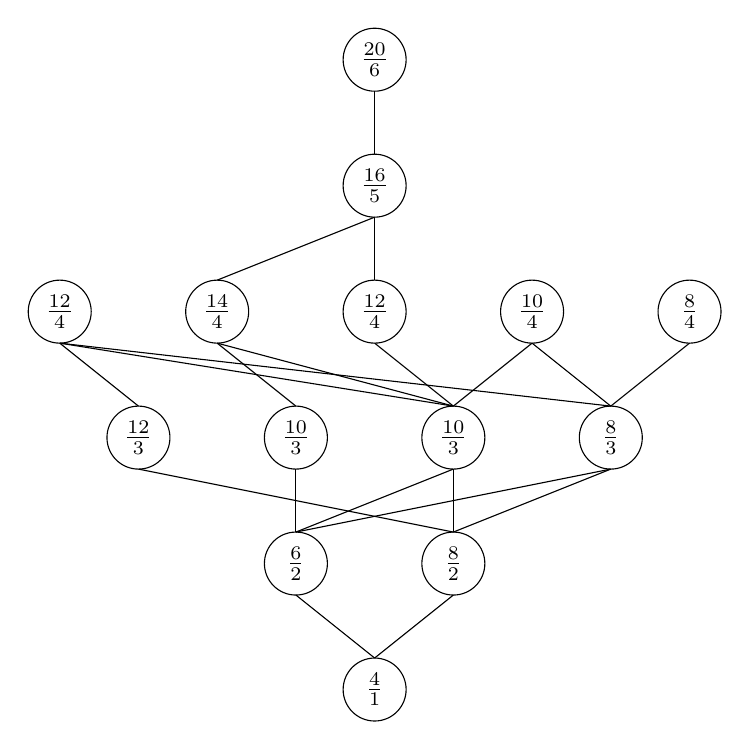
\begin{tikzpicture}
  [scale=.04,auto=left]
  
  \def\X{40}
  \def\Y{0}
  
  \def\x{\X -10}
  \def\y{\Y}
  
  \draw  (\x +10,\y +5) circle [radius=10cm] node {$\frac{4}{1}$};

  \def\x{\X -35}
  \def\y{\Y +40}
    
  \draw  (\x +10,\y +5) circle [radius=10cm] node {$\frac{6}{2}$};
  
  \draw  (\x +10,\y -5) -- (\x +35,\y -25);
  
  \def\x{\X +15}
  \def\y{\Y +40}
    
  \draw  (\x +10,\y +5) circle [radius=10cm] node {$\frac{8}{2}$};
  
  \draw  (\x +10,\y -5) -- (\x -15,\y -25);
  
  \def\x{\X -85}
  \def\y{\Y +80}
    
  \draw  (\x +10,\y +5) circle [radius=10cm] node {$\frac{12}{3}$};
  
  \draw  (\x +10,\y -5) -- (\x +110,\y -25);
  
  \def\x{\X -35}
  \def\y{\Y +80}
    
  \draw  (\x +10,\y +5) circle [radius=10cm] node {$\frac{10}{3}$};
  
  \draw  (\x +10,\y -5) -- (\x +10,\y -25);
  
  \def\x{\X +15}
  \def\y{\Y +80}
    
  \draw  (\x +10,\y +5) circle [radius=10cm] node {$\frac{10}{3}$};
  
  \draw  (\x +10,\y -5) -- (\x +10,\y -25);
  \draw  (\x +10,\y -5) -- (\x -40,\y -25);
  
  \def\x{\X +65}
  \def\y{\Y +80}
    
  \draw  (\x +10,\y +5) circle [radius=10cm] node {$\frac{8}{3}$};
  
  \draw  (\x +10,\y -5) -- (\x -40,\y -25);
  \draw  (\x +10,\y -5) -- (\x -90,\y -25);
  
  \def\x{\X -110}
  \def\y{\Y +120}
    
  \draw  (\x +10,\y +5) circle [radius=10cm] node {$\frac{12}{4}$};
  
  \draw  (\x +10,\y -5) -- (\x +35,\y -25);
  \draw  (\x +10,\y -5) -- (\x +135,\y -25);
  \draw  (\x +10,\y -5) -- (\x +185,\y -25);
  
  \def\x{\X -60}
  \def\y{\Y +120}
    
  \draw  (\x +10,\y +5) circle [radius=10cm] node {$\frac{14}{4}$};
  
  \draw  (\x +10,\y -5) -- (\x +35,\y -25);
  \draw  (\x +10,\y -5) -- (\x +85,\y -25);
  
  \def\x{\X -10}
  \def\y{\Y +120}
    
  \draw  (\x +10,\y +5) circle [radius=10cm] node {$\frac{12}{4}$};
  
  \draw  (\x +10,\y -5) -- (\x +35,\y -25);
  
  \def\x{\X +40}
  \def\y{\Y +120}
    
  \draw  (\x +10,\y +5) circle [radius=10cm] node {$\frac{10}{4}$};
  
  \draw  (\x +10,\y -5) -- (\x +35,\y -25);
  \draw  (\x +10,\y -5) -- (\x -15,\y -25);
  
  \def\x{\X +90}
  \def\y{\Y +120}
    
  \draw  (\x +10,\y +5) circle [radius=10cm] node {$\frac{8}{4}$};
  
  \draw  (\x +10,\y -5) -- (\x -15,\y -25);
  
  \def\x{\X -10}
  \def\y{\Y +160}
    
  \draw  (\x +10,\y +5) circle [radius=10cm] node {$\frac{16}{5}$};
  
  \draw  (\x +10,\y -5) -- (\x +10,\y -25);
  \draw  (\x +10,\y -5) -- (\x -40,\y -25);
  
  \def\x{\X -10}
  \def\y{\Y +200}
    
  \draw  (\x +10,\y +5) circle [radius=10cm] node {$\frac{20}{6}$};
  
  \draw  (\x +10,\y -5) -- (\x +10,\y -25);
\end{tikzpicture}
  \caption{The numbers \(h(G)\) for all cut-minimal graphs on 6 vertices}
  \label{figure2:Figure 2}
\end{figure}


\subsection{Deletions and additions of edges}
We will now investigate how the set \(T(G)\) (and so the constant \(h(G)\) as well) changes when we delete or add one or more edges in a given graph \(G\). This will give us some methods to determine that a given graph satisfying certain conditions is not a Cheeger graph.
\begin{defi}
Let \(G=([n],E)\) be a simple graph. For an edge \(e\in E\) we define the numbers:
\[
\psi_e^G:=|\{e'\in E\: :\: e'\text{ and }e\text{ share a vertex}\}|,
\]
where two edges \(e=(v_1,v_2)\) and \(e'=(v_3,v_4)\) are said to be sharing a vertex, if \(|(v_1,v_2)\cap (v_3,v_4)|=1\) and
\[
\phi_e^G:=|\{A\subseteq E\: :\: A\text{ is a triangle in }G\text{ and }e\in A\}|,
\]
where a triangle is a set of the type \(A=\{(v_1,v_2),(v_2,v_3),(v_3,v_1)\}\). If \(G\) contains no triangle, which is equivalent to \(\sum\limits_{e\in E}\phi_e^G=0\), then we call \(G\) \textbf{triangle-free}.
\end{defi}
\begin{lem}\label{lemma2}
Let \(G=([n],E)\) be a cut-minimal graph and \(e\in E\), then we have:
\begin{equation}
\psi_e^G\leq
\begin{cases}
n-3,&\text{ for }n\text{ odd}\notag\\
n-4,&\text{ for }n\text{ even}\notag
\end{cases}
\end{equation}
and
\begin{equation}
\phi_e^G\leq
\begin{cases}
\frac{n-3}{2},&\text{ for }n\text{ odd}\notag\\
\frac{n-4}{2},&\text{ for }n\text{ even}\notag
\end{cases}
\end{equation}
\begin{proof}
Let \(e:=(v_1,v_2)\), then we have \(\text{deg}_G(v_1),\text{deg}(v_2)\leq\left\lfloor\frac{n-1}{2}\right\rfloor\), so we get:
\[
\psi_e^G=\text{deg}_G(v_1)+\text{deg}_G(v_2)-2\leq2\left\lfloor\frac{n-1}{2}\right\rfloor-2
\]
Since \(2\left\lfloor\frac{n-1}{2}\right\rfloor=n-1\) for \(n\) odd and \(n-2\) for \(n\) even we get the claimed result.\\
The second part follows directly from the first one, since for each triangle containing \(e\), we have exactly two edges sharing a vertex with \(e\).
\end{proof}
\end{lem}
Since a Cheeger graph \(G\) can be characterized by the property that neither deleting edges from it nor adding edges to it (provided that the corresponding graph is still cut-minimal) nor a combination of both actions can decrease the number \(h(G)\), it might be helpful to know more about how those actions change \(h(G)\). The next Lemma gives exactly this information and the following statements then develop conditions which being satisfied by a certain graph guarantee that it is not a Cheeger graph.
\begin{lem}\label{lemma1}
Let \(G=([n],E)\) be a simple graph, \(e\in E\) and \(e'\in NE_G([n],[n])\). Then we have:
\begin{enumerate}
\item \(|T(G)|\leq |E|(n-2)-2\psi_e^G+2\phi_e^G\)
\item \(|T(G_e)|=|T(G)|-(n-2)+2(\psi_e^G-2\phi_e^G)\)
\item \(|T(G^{e'})|=|T(G)|+(n-2)-2(\psi_{e'}^{G^{e'}}-2\phi_{e'}^{G^{e'}})\)
\end{enumerate}
\begin{proof}
(1) The maximum number \(|T(G)|\) can become is obviously \(|E|(n-2)\), namely in the case when no two edges share a vertex. Now for an edge\\
\(e=(v_1,v_2)\in E\) contained in a triangle \(\{(v_1,v_2),(v_1,v_3),(v_2,v_3)\}\), we have \(\tau_e(v_3)=\frac{1}{3}\) instead of \(1\), so \(t(e)\) decreases at least by \(\frac{2}{3}\).
By 3 edges participating at each triangle, we then overall lose at least \(2\phi_e^G\).\\
If we have two edges \((v_1,v_2),(v_2,v_3)\in E\), such that \((v_1,v_3)\notin E\), meaning two edges which share a vertex but which are not contained in the same triangle, then we get \(\tau_{(v_1,v_2)}(v_3)=\tau_{(v_2,v_3)}(v_1)=0\) instead of \(1\), so overall we lose at least \(2(\psi_e^G-2\phi_e^G)\), since \(\psi_e^G-2\phi_e^G\) is the number of edges which share a vertex with \(e\) but which are not contained in the same triangle with \(e\).\\
All in all we get:
\[
|T(G)|\leq|E|(n-2)-2\phi_e^G-2(\psi_e^G-2\phi_e^G)=|E|(n-2)-2\psi_e^G+2\phi_e^G
\]
(2) The maximum number by which \(|T(G)|\) can decrease when deleting \(e\) from \(G\) is \(n-2\). This is the case when \(e\) is not connected to the rest of the graph. We do not have to consider the case when \(e\) is contained in a triangle because even though \(t(e)\) is smaller than \(n-2-\frac{2}{3}\) then, the numbers \(t(e')\) and \(t(e'')\) refering to the other two edges \(e'\) and \(e''\) contained in the triangle also decrease by \(\frac{1}{3}\) when deleting \(e\).
So, we still have to consider the case, when we have an edge \(e'\) sharing a vertex with \(e\) but not being contained in the same triangle with \(e\). Then \(|T(G)|\) decreases by one less than \(n-2\) and even increases by 1 when deleting \(e\), since \(t(e')\) increases by 1.\\
Hence, we get:
\[
|T(G_e)|=|T(G)|-(n-2)+2(\psi_e^G-2\phi_e^G)
\]
(3) By part (2) of this Lemma we have:
\[
|T(G)|=|T(G_{e'}^{e'})|=|T(G^{e'})|-(n-2)+2(\psi_{e'}^{G^{e'}}-2\phi_{e'}^{G^{e'}})
\]
which is equivalent to:
\[
|T(G^{e'})|=|T(G)|+(n-2)-2(\psi_{e'}^{G^{e'}}-2\phi_{e'}^{G^{e'}}).
\]
\end{proof}
\end{lem}
\begin{prop}\label{proposition1}
Let \(G=([n],E)\) be a simple graph. If there exists an edge \(e\in E\), such that \(2(|E|-1)\psi_e^G-2(2|E|-1)\phi_e^G<0\), then we have \(h(G_e)<h(G)\).
\begin{proof}
By Lemma \ref{lemma1} (1) we get:
\begin{doublespace}
\begin{align}
&\quad\quad\quad\:\, |E|(n-2)-(2\psi_e^G-2\phi_e^G)\geq |T(G)|\notag\\
&\Longleftrightarrow\quad |E||T(G)|-|E|(n-2)+(2\psi_e^G-2\phi_e^G)\leq |T(G)|(|E|-1)\notag\\
&\Longleftrightarrow\quad \frac{|E||T(G)|-|E|(n-2)+(2\psi_e^G-2\phi_e^G)}{|E|(|E|-1)}\leq\frac{|T(G)|(|E|-1)}{|E|(|E|-1)}\notag\\
&\Longleftrightarrow\quad \frac{|T(G)|-(n-2)}{|E|-1}+\frac{2\psi_e^G-2\phi_e^G}{|E|(|E|-1)}\leq\frac{|T(G)|}{|E|}=h(G)
\end{align}
\end{doublespace}
and by Lemma \ref{lemma1} (2) we get:
\begin{align}
h(G_e)=\frac{|T(G)|-(n-2)}{|E|-1}+\frac{2\psi_e^G-4\phi_e^G}{|E|-1}
\end{align}
Now consider:
\begin{doublespace}
\begin{align}
&\quad\quad\quad\:\, 2(|E|-1)\psi_e^G-2(2|E|-1)\phi_e^G<0\notag\\
&\Longleftrightarrow\quad 2(|E|-1)\psi_e^G-(4|E|-2)\phi_e^G<0\notag\\
&\Longleftrightarrow\quad 2(|E|-1)\psi_e^G-4|E|\phi_e^G+2\phi_e^G<0\notag\\
&\Longleftrightarrow\quad 2|E|\psi_e^G-4|E|\phi_e^G<2\psi_e^G-2\phi_e^G\notag\\
&\Longleftrightarrow\quad \frac{2\psi_e^G-4\phi_e^G}{|E|-1}<\frac{2\psi_e^G-2\phi_e^G}{|E|(|E|-1)}\notag
\end{align}
\end{doublespace}
So, by (1) and (2) we have:
\[
h(G_e)<h(G)
\]
\end{proof}
\end{prop}
\begin{expl}
Let \(G=([n],E)\) be a simple graph containing a triangle, which is only connected to the rest of the graph via one vertex or isolated, meaning a set \(\{(v_1,v_2),(v_2,v_3),(v_1,v_3)\}\subseteq E\), such that \(\text{deg}_G(v_1)=\text{deg}_G(v_2)=2\), then \(G\) is not a Cheeger graph as follows. We set \(e:=(v_1,v_2)\), then we have \(\phi_e^G=1\) and \(\psi_e^G=2\). This gives us:
\[
2(|E|-1)\psi_e^G-2(2|E|-1)\phi_e^G=4(|E|-1)-2(2|E|-1)=-2<0
\]
and by Proposition \ref{proposition1} we get:
\[
h(G_e)<h(G),
\]
so \(G\) can not be a Cheeger graph.
\end{expl}
Now we want to generalize the second and third part of Lemma \ref{lemma1} to a situation where we consider more than only one edge being deleted or added.
\begin{lem}\label{lemma3}
Let \(G=([n],E)\) be a simple graph and \(e_1,\ldots,e_k\in E\), then we have:
\[
|T(G_{e_1,\ldots,e_k})|=|T(G)|-k(n-2)+2(\sum\limits_{i=1}^k\psi_{e_i}^{G_{e_1,\ldots,e_{i-1}}}-2\sum\limits_{i=1}^k\phi_{e_i}^{G_{e_1,\ldots,e_{i-1}}})
\]
In this formula we set \(G_{e_0}=G\) to avoid writing it in a more complicated way.\\
For \(e_1,\ldots,e_k\in NE_G([n],[n])\) we have:
\[
|T(G^{e_1,\ldots,e_k})|=|T(G)|+k(n-2)-2(\sum\limits_{i=1}^k\psi_{e_i}^{G^{e_1,\ldots,e_i}}-2\sum\limits_{i=1}^k\phi_{e_i}^{G^{e_1,\ldots,e_i}})
\]
\begin{proof}
By Lemma \ref{lemma1} (2) we get:
\begin{align}
|T(G_{e_1,\ldots,e_k})|&=|T(G_{e_1,\ldots,e_{k-1}})|-(n-2)+2(\psi_{e_k}^{G_{e_1,\ldots,e_{k-1}}}-2\phi_{e_k}^{G_{e_1,\ldots,e_{k-1}}})\notag\\
&=|T(G_{e_1,\ldots,e_{k-2}})|-(n-2)+2(\psi_{e_{k-1}}^{G_{e_1,\ldots,e_{k-2}}}-2\phi_{e_{k-1}}^{G_{e_1,\ldots,e_{k-2}}})\notag\\
&\quad-(n-2)+2(\psi_{e_k}^{G_{e_1,\ldots,e_{k-1}}}-2\phi_{e_k}^{G_{e_1,\ldots,e_{k-1}}})\notag\\
&=|T(G_{e_1,\ldots,e_{k-2}})|-2(n-2)\notag\\
&\quad+2(\psi_{e_{k-1}}^{G_{e_1,\ldots,e_{k-2}}}+\psi_{e_k}^{G_{e_1,\ldots,e_{k-1}}}-2(\phi_{e_{k-1}}^{G_{e_1,\ldots,e_{k-2}}}+\phi_{e_k}^{G_{e_1,\ldots,e_{k-1}}}))\notag
\end{align}
so inductively we have:
\[
|T(G_{e_1,\ldots,e_k})|=|T(G)|-k(n-2)+2(\sum\limits_{i=1}^k\psi_{e_i}^{G_{e_1,\ldots,e_{i-1}}}-2\sum\limits_{i=1}^k\phi_{e_i}^{G_{e_1,\ldots,e_{i-1}}})
\]
The second part works analogously using Lemma \ref{lemma1} (3). 
\end{proof}
\end{lem}
\begin{prop}\label{proposition2}
Let \(G=([n],E)\) be a simple graph. If there exist edges \(e_1,\ldots,e_k\in E\) and \(e\in E\) such that:
\[
\frac{2(\sum\limits_{i=1}^k\psi_{e_i}^{G_{e_1,\ldots,e_{i-1}}}-2\sum\limits_{i=1}^k\phi_{e_i}^{G_{e_1,\ldots,e_{i-1}}})}{|E|-k}<\frac{k(2\psi_e^G-2\phi_e^G)}{|E|(|E|-k)},
\]
then we have:
\[
h(G_{e_1,\ldots,e_k})<h(G)
\]
\begin{proof}
By Lemma \ref{lemma1} (1) we get:
\begin{doublespace}
\begin{align}
&\quad\quad\quad\:\, |E|(n-2)-(2\psi_e^G-2\phi_e^G)\geq |T(G)|\notag\\
&\Longleftrightarrow\quad |E||T(G)|-k|E|(n-2)+k(2\psi_e^G-2\phi_e^G)\leq |T(G)|(|E|-k)\notag\\
&\Longleftrightarrow\quad \frac{|E||T(G)|-k|E|(n-2)+k(2\psi_e^G-2\phi_e^G)}{|E|(|E|-k)}\leq\frac{|T(G)|(|E|-k)}{|E|(|E|-k)}\notag\\
&\Longleftrightarrow\quad \frac{|T(G)|-k(n-2)}{|E|-k}+\frac{k(2\psi_e^G-2\phi_e^G)}{|E|(|E|-k)}\leq\frac{|T(G)|}{|E|}=h(G)
\end{align}
\end{doublespace}
and Lemma \ref{lemma3} gives us:
\[
h(G_{e_1,\ldots,e_k})=\frac{|T(G)|-k(n-2)}{|E|-k}+\frac{2(\sum\limits_{i=1}^k\psi_{e_i}^{G_{e_1,\ldots,e_{i-1}}}-2\sum\limits_{i=1}^k\phi_{e_i}^{G_{e_1,\ldots,e_{i-1}}})}{|E|-k}
\]
So, by (3) and the assumption we have:
\[
h(G_{e_1,\ldots,e_k})<h(G)
\]
\end{proof}
\end{prop}

\subsection{Adding vertices to Cheeger graphs}
After we studied how adding or deleting edges in a cut-minimal graph \(G\) affects its constant \(h(G)\) we are now interested in the consequences of adding a vertex to \(G\). We will find out that in the most cases the property of being a Cheeger graph will be destroyed by this action. Using this knowledge we can construct a lower bound on the number of edges in Cheeger graphs holding in the most cases.
\begin{lem}\label{lemma4}
Let \(G=([n],E)\) be a cut-minimal graph, then we have:
\[
h(i_n(G))=h(G)+1
\]
\begin{proof}
Adding an isolated vertex to a graph \(G=([n],E)\) obviously increases \(|T(G)|\) by \(|E|\), so we get:
\[
h(i_n(G))=\frac{|T(G)|+|E|}{|E|}=\frac{|T(G)|}{|E|}+\frac{|E|}{|E|}=h(G)+1
\]
\end{proof}
\end{lem}
A direct consequence of this relation is that if \(n\) is not divisible by 3, Cheeger graphs in \(CMG(n)\) can not appear as an embedding of graphs from \(CMG(n-1)\).
\begin{prop}\label{proposition4}
For all \(G\in CMG(n)\), such that \(3\nmid n\) the graph\\
\(i_n(G)\in CMG(n+1)\) is not a Cheeger graph.
\begin{proof}
We only need to consider Cheeger graphs in \(CMG(n)\), since for any\\
\(G\in CMG(n)\) which is not a Cheeger graph, there exists a graph \(G'\in CMG(n)\), such that \(h(G')<h(G)\), so by Lemma \ref{lemma4} we get:
\[
h(i_n(G'))=h(G')+1<h(G)+1=h(i_n(G))
\]
Let now \(G\in CMG(n)\) be a Cheeger graph. Then by a result from \cite{1} we get:
\[
\frac{n}{3}\leq h(G)\leq\left\lceil\frac{n}{3}\right\rceil
\]
which implies that:
\[
h(i_n(G))=h(G)+1\geq\frac{n}{3}+1\geq\left\lceil\frac{n+1}{3}\right\rceil,
\]
where the last inequality is sharp if and only if \(3\nmid n\).\\
So, if \(3\nmid n\) then \(i_n(G)\) is not a Cheeger graph, since by \cite{1} we have:
\[
h_1(\Delta^{[n+1]})\leq\left\lceil\frac{n+1}{3}\right\rceil<h(i_n(G))
\]
\end{proof}
\end{prop}
We even have a similar version of the previous statement if \(n\) is divisible by 3 with the restriction that \(n+1\) must not be a power of 2.
\begin{prop}\label{proposition5}
Let \(G\in CMG(n)\), such that \(3\mid n\) and \(n+1\neq2^t\) for some \(t\in\mathbb{N}\). Then \(i_n(G)\) is not a Cheeger graph.
\begin{proof}
Since \(n\) is divisible by 3 we have \(h(G)=\frac{n}{3}\) by \cite{1} and so we get\\
\(h(i_n(G))=\frac{n}{3}+1\) by Lemma \ref{lemma4}. Now, since \(n+1\) is not a power of 2 we also know that \(h_1(\Delta^{[n+1]})=\frac{n+1}{3}\) by \cite{1}. Hence, we have:
\[
h(i_n(G))>h_1(\Delta^{[n+1]})
\]
\end{proof}
\end{prop}
Combining the last two statements, we can calculate a lower bound for the number of edges in Cheeger graphs, except for the case when the number of vertices \(n\) is a power of 2 and \(n-1\) is divisible by 3.
\begin{prop}
Let \(G=([n],E)\) be a Cheeger graph, such that \(n\) is not a power of 2 or \(n-1\) is not divisible by 3. Then we have \(|E|\geq\left\lceil\frac{n-1}{2}\right\rceil\).
\begin{proof}
Assume we have \(|E|<\left\lceil\frac{n-1}{2}\right\rceil\). Then by Theorem \ref{theorem2} and since \(G\) must contain an isolated vertex, there exists a graph \(G'\in CMG(n-1)\), such that \(i_{n-1}(G')=G\). Now if we have \(n\neq 2^t\) for some \(t\in\mathbb{N}\), then \(G\) is not a Cheeger graph, since we either get \(3\nmid n-1\) and we are done by Proposition \ref{proposition4} or we get \(3\mid n-1\) and we are done by Proposition \ref{proposition5}. On the other hand, if we have \(n=2^t\) but \(3\nmid n-1\), then we immediately see that \(G\) is not a Cheeger graph by Proposition \ref{proposition4}.
\end{proof}
\end{prop}